\documentclass[]{report}
%\usepackage[sc]{computermodern} % Use the Palatino font
%\usepackage[utf8x]{inputenc}
%\usepackage[T1]{fontenc} % Use 8-bit encoding that has 256 glyphs
%\linespread{1.05} % Line spacing - Palatino needs more space between lines
\usepackage{microtype} % Slightly tweak font spacing for aesthetics
\usepackage{graphicx,xcolor}
\usepackage{subfigure}

\usepackage[hmarginratio=1:1,top=25mm,columnsep=20pt,lmargin=20mm,rmargin=20mm,bmargin=20mm]{geometry} % Document margins
\usepackage{multicol} % Used for the two-column layout of the document
%\usepackage[hang, small,labelfont=bf,up,textfont=it,up]{caption} % Custom captions under/above floats in tables or figures
\usepackage{booktabs} % Horizontal rules in tables
\usepackage{float} % Required for tables and figures in the multi-column environment - they need to be placed in specific locations with the [H] (e.g. \begin{table}[H])
\usepackage{hyperref} % For hyperlinks in the PDF

\usepackage{lettrine} % The lettrine is the first enlarged letter at the beginning of the text
\usepackage{paralist} % Used for the compactitem environment which makes bullet points with less space between them

\usepackage{abstract} % Allows abstract customization
\renewcommand{\abstractnamefont}{\normalfont\bfseries} % Set the "Abstract" text to bold
%\renewcommand{\abstracttextfont}{\normalfont\small\itshape} % Set the abstract itself to small italic text

\usepackage{titlesec} % Allows customization of titles
\renewcommand\thesection{\Roman{section}} % Roman numerals for the sections
\renewcommand\thesubsection{\Roman{subsection}} % Roman numerals for subsections
%\titleformat{\section}[block]{\large\scshape\centering}{\thesection.}{1em}{} % Change the look of the section titles
%\titleformat{\subsection}[block]{\large}{\thesubsection.}{1em}{} % Change the look of the section titles

%\usepackage{fancyhdr} % Headers and footers
%\pagestyle{fancy} % All pages have headers and footers
%\fancyhead{} % Blank out the default header
%\fancyfoot{} % Blank out the default footer
%\fancyhead[C]{} % Custom header text
%\fancyfoot[RO,LE]{\thepage} % Custom footer text

\usepackage[percent]{overpic}
\raggedbottom


% Title Page
\title{\textbf{Guide for VBF Analysis Through ANN}\\
	(Procedure Adopted on CMS-AN-18-120)}
\author{Miqueias Melo de Almeida}


\begin{document}
\maketitle

\begin{abstract}
This guide brings a brief description of the codes developed for the isolated VBF XS measurement using the reduced ntuples framework developed by prof. Nicola De Filippis. The guide covers the procedures developed for: building up Artificial Neural Networks (ANNs) using Keras, estimating Z+X background (thanks to Reham) and producing a statistical Analysis using Higgs Combine tool. This guide will describe what does and how to use the codes contained into the AnalysisCodes folder (which should contain this guide). Each python codes contains some explanation of their commands line so that the user can find more details. Feel free to also modify the structure of the codes according to your needs.
\end{abstract}

\section{ANNs Training using Keras an RECAS Computing Farm}
In order to develop the Artificial Neural Networks (ANNs) a framework was developed using Keras, which is a set of python libraries that allows one to create any ANN structure (as known so far) using few lines of codes (all the objects defined using Keras can be fully hand-coded but this is time consuming and not the focus for Physics). For full details see \url{https://keras.io/} which is the Keras web page containing the full documentation about all functions and classes defined within this package. Keras needs another set of python libraries which handled the tensorial operations associated to the building and training of a ANN. Nowadays Keras accept two of those: the Tensorflow (which should become the official one in the future) and Theano (which is no longer maintained by its community - it'll become obsolete at some point). These configuration issues are not a trouble for the user anymore because CERN has adopted Keras into his set of libraries within the cvmfs environment. So, in order to have Keras working at RECAS one just needs to run the following command: \textbf{source /cvmfs/sft.cern.ch/lcg/views/LCG\_94/x86\_64-slc6-gcc62-opt/setup.sh}. 

Once Keras is ready the first thing to do is to prepare the datasets (events from MC) to be used as examples, to train the ANNs, and as probes, to test them. So, a python dictionary is a good object to store arrays containing subset of information from the reduced ntuples. The \textbf{Keras/FormatROOTs.py} and \textbf{Keras/runFormatROOTs.sh} macros are used for this purpose. What it does could be done in a single run but since it takes time is better to make this separately just once and not every time you run an ANN training. The runFormatROOTs.sh simplifies the running procedure of FormatROOTs.py which takes some commands line. The runFormatROOTs.sh is where the user should specify the list of MC files which one wants to use, the number of jets (since for VBF 2016 analysis there were created a separated ANN for 2 and 3 jets case). Fig.~\ref{fig:formatimputssh} shows how that macro looks like. Its commands line are:
\begin{itemize}
	\item infile: receives a list of the MC files name;
	\item outfile: the name of the output file used into Keras (the dictionary created by the code);
	\item njets: specifies the number of jets (one can creates separated dictionaries for each case, please see the FormatROOTs.py to understand how the jets are handled);
	\item maxsubjets and nsubjets: it can be ignored if there's no interest in studying jet image (leave the options set like in the figure for fast running);
	\item keys: are the names one wants to label each MC file within the dictionary;
	\item tags: are the names used to identify the MC files specified into the file passed to infile command line (be aware, they must be different for each file in order to avoid double counting - note that in the figure they are the names of the MC files).
\end{itemize}

\begin{figure}
	\label{fig:formatimputssh}
	\centering
	\caption{A view of runFormatROOTs.sh macro.}
	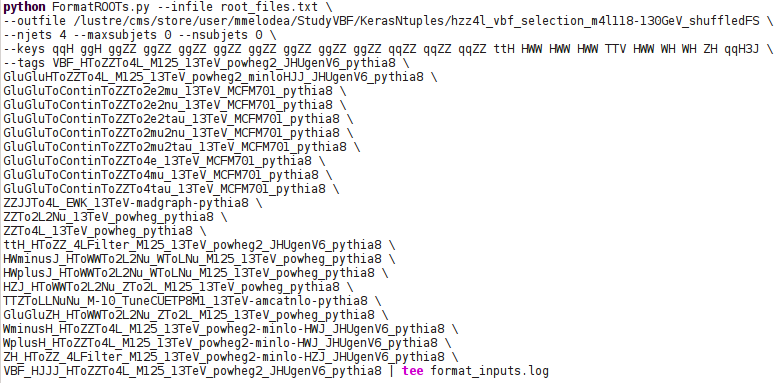
\includegraphics[scale=0.8]{figs/formatimputssh}
\end{figure}

After running runFormatROOTs.sh macro (like "bash runFormatROOTs.sh"), which takes about 10 min, a file with ".pkl" extension will be created in the folder where the macro was ran. Just as quick description of this kind of file, the python dictionary is a container storing arrays which indexes can be "names". So, for instance, once the dictionary is loaded, the $p_{T}$ of the first lepton (which are sorted by $p_{T}$) can be accessed in a event using the syntax "array[0]['f\_lept1\_pt']" (the labels at the moment have been defined as the branch names of the variables stored in the TTree in the reduced ntuples). The splitting of the events have been defined in such way that one can get a certain fraction of each MC file and the events are randomized in order to mix the four-lepton final states and the MC process. 

The next step is to run the ANNs training. With Keras the user writes his (her) own code and there are several parameters which needs to be set up. This means there are several configurations one can build up and, writing the code and training each of them separately is for sure not efficient (and also don't allow great coverage of the models that can be built). In order to be able to run several ANN models in parallel the \textbf{Keras/runEvaluateNeuralNetwork.sh} and \textbf{Keras/EvaluateNeuralNetwork.py} macros were created. The work similarly to previous ones. The ".sh" script is where the user specifies commands line used by the python code. The commands line accepted at this stage are (please, see the appendix to understand the meaning of the parameters here):
\begin{itemize}
	\item infile: receives the address of the input file (the pkl dictionary);
	\item keys: receives the labels of the MC processes that one wants to use in the training (the MC not specified is not used, even if it's contained into the dictionary);
	\item nninputs: receives the variables to be used as inputs for the neural network;
	\item layers: receives the ANN topology (for instance, 10 10 10 means a ANN with 3 layers containing 10 neurons each);
	\item batchsize: receives the size of the batch sample of events used to train the events;
	\item patience: receives the number of epochs to keep training without improvement;
	\item scaletrain: receives a label to specify which kind of weight to be used when scaling the contribution of each MC process during the training (see appendix for more detail on the reason to use this option);
	\item neuron: receives the type of neuron to be used (the activation function, see Keras web page to see some examples). The ReLU and SeLU type are recommended.
\end{itemize}

\begin{figure}
	\label{fig:evaluateneuralnetworksh}
	\centering
	\caption{A view of runEvaluateNeuralNetwork.sh macro.}
	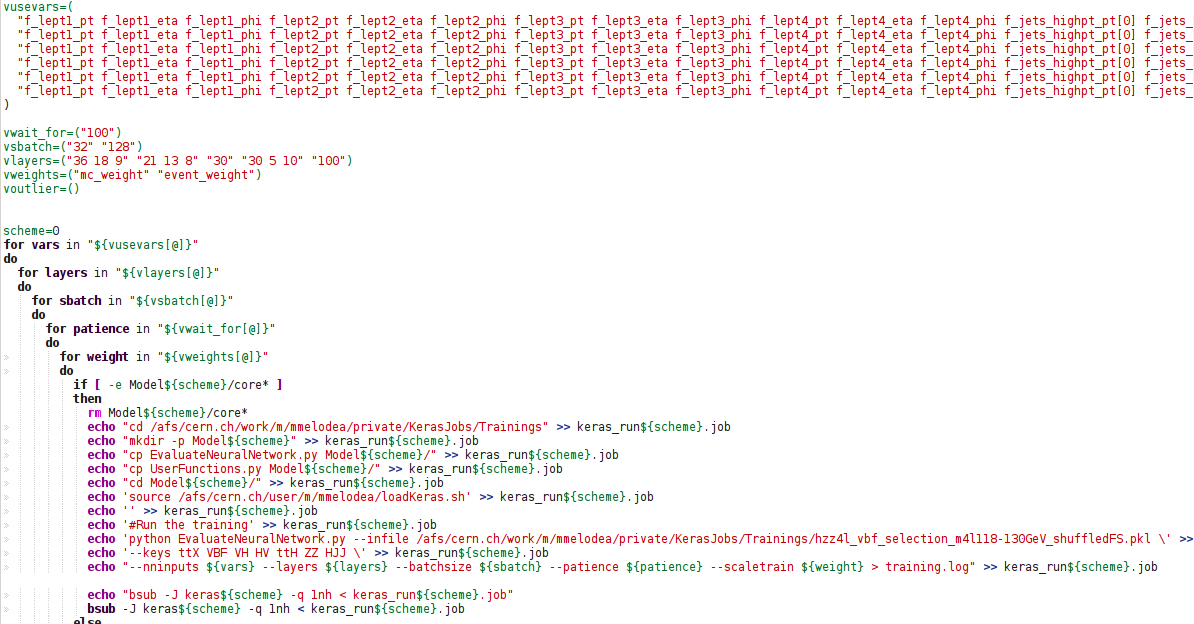
\includegraphics[angle=90,scale=0.7]{figs/evaluateneuralnetworksh}
\end{figure}

As it can be seen in Fig.~\ref{fig:evaluateneuralnetworksh}, the ".sh" script makes a loop over any configuration the user wants and send multiples jobs to RECAS computing farm. It just needs to be specified in the arrays in the script. Once a jobs is finished, the folder containing such job will contain a set of plots which shows the performance of the trained ANN (which by the way, allows the user to check if there was overfitting on the ANN training - note that this trouble is avoided when ModelCheckPoint parameter, which is default in the macros, is used in Keras). Since the VBF analysis has the MELA discriminant from CMS, the plots show a comparison with MELA performance in the same MC events used to test the trained ANN. The script \textbf{Keras/checkTrainings.py} can be used to run over the dictionary also created at this stage. This dictionary contains variables describing the performance of each ANN and the script will outputs such performances in terms of the $\epsilon.\pi$ (efficiency.purity) and the significance of the signal. 

Once the training of the ANN training is finished there will be a file with ".h5" extension in the jobs folder. This file is the one which contains the ANN function. This file can't be used to run a on-flying analysis. If the user wants to use it, then the procedure is to use a python code to store the ANN outputs per event into a new TTree. The \textbf{Keras/exportNetwork.py} macro was created to convert the Keras h5 format into a ".h" macro, which allows one to plug such file into another analysis codes. This macro is executed as (see an example of the ".h" file in the Keras folder)

\textbf{python exportNetwork.py --infile keras\_model --outfile output\_file}.

{\color{red}\textbf{ATTENTION}}, at the time of this guide, the Keras package doesn't have the functionality to export the trained ANN in a given format that can be used on fly. The exportNetwork.py macro is not optimal and thus can't convert Keras ANNs trained using Dropout or other activation functions different from ReLU and SeLU.

\section{The Z+X Estimation}
The Z+X estimation follows very close the procedure adopted in the analysis reported at AN-16-328 and few modifications were introduced in the codes in order to store the events used in the Z+X estimation. Such events present the same variables as the MC files which allows one to use them in the ANN training and for deriving the Z+X shape via the ANNs.

The first step for deriving the Z+X background is to compute the so called fake rates. In order to do that one needs to select samples of Z+lepton, where the Z are build using two tight leptons and the third lepton can be loose or tight (see AN-16-328 or AN-18-120 for the requirements defining the loose and tight leptons). The fake rate is then the ratio between the number of events with the third lepton being tight and the number of events with the third lepton being loose. For the VBF analysis it was decided to compute the fake rate as a function of the third lepton $p_{T}$ and $\eta$. The second step is the application of the fake rate into two control regions of four-lepton events composed of two tight leptons plus, either two loose leptons (2P2F CR) or one tight and one loose lepton (3P1F CR).

The \textbf{ZplusX/ComputeFRandCRsOS.cc} macro is the macro which does this two steps in a single run. This macro needs to be compiled by running the script \textbf{ZplusX/compileference.sh}, which will produce the executable \textbf{ZplusX/ComputeFRandCRs}. This executable receives as arguments the name of the big ntuples (small ntuples obtained from MiniAODs and the ones from which the reduced ntuples are produced), the number of events before and after the HLT selections and the XS of the given process (if Data the argument should be set to 1). The script \textbf{ZplusX/submit\_jobs.sh} can be used to send jobs to RECAS computing farm. Once the jobs are finished, then one needs to prepare the datasets for the Z+X estimation (see the \textbf{ZplusX/*Spring16*.txt}). The \textbf{ZplusX/IncludeKeras.cc} macro is used to insert in the TTrees produced for the Z+X estimation the ANN output for each event. 

The Z+X estimation uses an equation (which can be found in the CMS HZZ4L ANs) that combines the contribution coming from two components: one from 2P2F and one from 3P1F. $m_{4l}$ shapes in each of these CRs can be derived using the \textbf{ZplusX/plotCRs.cc} macro (run root -l -q $plotCRs.cc\setminus(\setminus"vbf\setminus",\setminus"4mu\setminus",\setminus"FRmap.root\setminus"\setminus)$ to plot those shapes\footnote{The "vbf" label can be replaced by "smhiggs" in order to plot the same shapes from the events after SM Higgs selections.}), where vbf stands for VBF-SR, 4mu is the final state and FRmap.root is the file containing the fake rate map) while the FR maps can be plotted using the \textbf{ZplusX/plotFR.cc} macro (run root -l $plotFR.cc\setminus(\setminus"MergedData.root\setminus",\setminus"MergedZZ.root\setminus"\setminus)$ to plot the FR maps), where MergedData.root and MergedZZ.root stands for the files created after merging the data and ZZ files produced when running the ComputeFRandCRs executable). 

In order to properly derive yields and shapes, the Z+X equation have been implemented through histograms and the estimation ultimately uses only Data and MC events from ZZ processes. The macro plotCRs.cc is the one to be used, which will outputs on the terminal screen the values of Z+X in each four-lepton final state ($4\mu$, $4e$, $2e2\mu$ and $2\mu2e$). The final numbers into $4l$ were estimated by combining the yields derived in each final state. The $4l$ yields are the sum of the yields in each final state and its uncertainty has been estimated by quadratically summing their uncertainty. Also, note that, for final states where the muons are the loose leptons ($4\mu$ and $2e2\mu$) the Z+X is not derived from the full equation but instead it is just the component coming from 2P2F. One can compute the final Z+X yields and uncertainties by hand but there's is the \textbf{ZplusX/computeFinalZX.cc} which can be used for that, the user just needs to state on it the yields given by the plotCRs.cc macro.

The derivation of Z+X shapes for a given trained ANN is straightforward since the same histograming procedure mentioned above is executed. The events selected in each of the CRs are just fed to the ANN and the histograms are used. Please, check the plotCRs.cc macro and the Z+X equation to better understand this procedure. Since the events selection for the Z+X estimation takes time, the \textbf{ZplusX/IncludeKeras.cc} macro has been created to produce a new version of the output files of the ComputeFRandCRs executable, containing the ANN output value for each event. So, this macro should be ran before the plotCRs.cc macro. 

Once these steps have been executed the last thing to do is just to merge the files created. The \textbf{ZplusX/combineOSSF.sh} can be used for that. Please, take a look to see how to properly merge the files in order to have the appropriate histograms.

\section{Statistical Analysis}
The statistical analysis has some complex theoretical background and it will not be mentioned here. For complete details please check the CMS-AN-18-120 and the Higgs Combine tool web page. The steps discussed in this section comprehends then, the proposed procedure to estimate the uncertainty on the 3rd jet in the events, the uncertainty on the ANN shape due to the uncertainty on its inputs and the procedures adopted to get some statistical results (focused here on HybridNew method which is the recommended one by the LHC Higgs Combination Group). The summary of the commands and procedures from Z+X estimation to the obtainment of limits are (note that you can adapt them, they just reflect how they were executed previously):

\begin{itemize}
\item[1] run plotCR.cc to generate Z+X shapes;
\item[1.1] copy files to vbf folder and make the merging of the generated files running combineOS*;
\item[2] run plotObjectsProperties.cc to generate Data and remaining BKGs shapes and, create a file including them and Z+X;
\item[2.2] copy the Histograms.root file locally;
\item[3] run plot3rdJetUncertainty.cc to generate the ANN shapes for each channel in the Njets3 category from VBF-H2J and VBF-H3J, getting their ratio (= to the uncertainty)
\item[4] run checkUnc1Sigma*.cc to generate all process and their +/- 1sigma shifts (first set of files used in the limits procedure);
\item[4.1] merge the generated files (hadd Distribution*.root)
\item[5] run create\_datacards.sh, which calls the genInputs*.py creating the *.txt and *.root datacards needed for limits;
\item[6] run combine\_cards.sh to combine the cards using combine tool;
\item[7] run Limits:
\item[7.1] Best fit: combine ./../combinedCard\_Higgs125GeV\_VBFStudy\_k57nj2\_k24nj3\_4l.txt -M FitDiagnostics --plots --saveOverallShapes --saveWithUncertainties >$\&$ combineResults.log
\item[7.2] Best fits: combine ./../combinedCard\_Higgs125GeV\_VBFStudy\_k57nj2\_k24nj3\_4l.txt -M ChannelCompatibilityCheck --saveFitResult >$\&$ combineResults.log
\item[7.3] Obs Likelihood: combine ./../combinedCard\_Higgs125GeV\_VBFStudy\_k57nj2\_k24nj3\_4l.txt -M MultiDimFit -n Obs --algo=grid --points 300 >$\&$ combineResults.log
\item[7.4] Exp Likelihood: combine ./../combinedCard\_Higgs125GeV\_VBFStudy\_k57nj2\_k24nj3\_4l.txt -M MultiDimFit -n Exp --algo=grid --points 300 -t -1 --expectSignal=1 >$\&$ combineResults.log
\item[7.5] Impact plot:
\item[7.5.1] text2workspace.py ../combinedCard\_Higgs125GeV\_VBFStudy\_k57nj2\_k24nj3\_4l.txt -m 125
\item[7.5.2] python combineTool.py -M Impacts -d ../combinedCard\_Higgs125GeV\_VBFStudy\_k57nj2\_k24nj3\_4l.root -m 125 --doInitialFit --robustFit 1
\item[7.5.3] python combineTool.py -M Impacts -d ../combinedCard\_Higgs125GeV\_VBFStudy\_k57nj2\_k24nj3\_4l.root -m 125 --robustFit 1 --doFits
\item[7.5.4] python combineTool.py -M Impacts -d ../combinedCard\_Higgs125GeV\_VBFStudy\_k57nj2\_k24nj3\_4l.root -m 125 -o impacts\_obs\_4l\_k57nj2\_k24nj3.json
\item[7.5.5] python plotImpacts.py -i impacts\_obs\_4l\_k57nj2\_k24nj3.json -o impacts\_obs\_4l\_k57nj2\_k24nj3
\item[7.6] ExpHybridLimMedian: combine ./../combinedCard\_Higgs125GeV\_VBFStudy\_k57nj2\_k24nj3\_4l.txt -M HybridNew --LHCmode LHC-limits -H AsymptoticLimits -T 50000 --expectedFromGrid=0.5 --expectSignal=1 >$\&$ combineResults.log
\item[7.7] ExpHybridLimObs: combine ./../combinedCard\_Higgs125GeV\_VBFStudy\_k57nj2\_k24nj3\_4l.txt -M HybridNew --LHCmode LHC-limits -H AsymptoticLimits -T 50000 >$\&$ combineResults.log
\item[7.8] ExpHybridSigMedian: combine ./../combinedCard\_Higgs125GeV\_VBFStudy\_k57nj2\_k24nj3\_4l.txt -M HybridNew --LHCmode LHC-significance -H Significance -T 50000 --expectedFromGrid=0.5 --expectSignal=1 >$\&$ combineResults.log
\item[7.9] ObsHybridSigMedian: combine ./../combinedCard\_Higgs125GeV\_VBFStudy\_k57nj2\_k24nj3\_4l.txt -M HybridNew --LHCmode LHC-significance -H Significance -T 50000 >$\&$ combineResults.log	
\end{itemize}

For plotting there are some macros in the package and the use as inputs the datacard root files created for the statistical analysis and the root files created by combine when running the previous commands. Their name should be self-explaining with the terminology used within Higgs Combine tool. For extra details on this steps please see the recent workshop realized at Fermilab (some codes were derived based on it): \url{https://indico.cern.ch/event/747340/timetable/}.


\appendix
\section{Appendix: Keras Parameters Meaning}
\begin{itemize}
	\item \textbf{pre-processing}: it is a usual practice in Machine Learning field to apply some operation in the NN inputs in order to standardize them (keep them in the same range of values for instance). In the scans done the pre-processing showed negligible effects and it was decided to not adopt such procedure for further studies. Note that, when pre-processing is applied in the training it will be need to also apply the same procedure when using the trained NN (otherwise the results will be mistaken, since the NN are expecting preprocessed inputs). One also should note that preprocessing changes the input variables what may destroy the possibility of the NN reconstruct some important property(e.g. invariant masses);
	\item \textbf{Topology}: the architecture of the NN, that is, the number of hidden layers, neurons and the neuron type. In Keras there are several types of neuron which even includes possible learning parameters (during training). The \textit{Rectified Linear Unity} (ReLU) is the most recommended due to its property of non-vanishing gradient;
	\item \textbf{Batch size}: the number of events in a subset from the training set used to compute the gradients and update the \textbf{$w_{i}$}'s and \textbf{$b$} in each neuron;
	\item \textbf{Epochs}: the number of iterations over the full training set. The total number of iterations is a combination of the size of the training set, the batch size and the number of epochs. For instance, setting a training of 10 epochs and a batch size of 10 for a training set size of 100 means that Keras performs $10^{2}$ updates on the \textbf{$w_{i}$}'s and \textbf{$b$}'s;
	\item \textbf{Early stop}: a parameter to set the number of epochs which Keras should wait if not improvement in the loss function is observed. If still not improvement is seen after that number of epochs the training is stopped;
	\item \textbf{Minimizer}: is the method to compute the gradients. There are several options in Keras (SGD, Adam, RMSprop, etc.) and after testing most of them it was decided to keep Adam. Adam stands for Adaptive Momentum and has the property of fast convergence due to a NN updating directed towards the loss function minimum. This minimizer is widely applied in ML studies;
	\item \textbf{Scaling}: Keras allows one to scale the loss function by some weight that can be independent for each training example or the same for a entire class (signal or background, for instance). It was tested the impact of using the expected yield (XS) of each process and the individual weights of each event ($\sigma.\epsilon.BR$).
	\end{itemize}

\section{Appendix: Scaling Events Contribution in the Training}
In the beginning of this analysis the NN trainings were carried out without taking into account any kind of event weight. In such way all events are seen by the NN in an equal basis. Keras has some features that allows one to include scale factor (example weight) which are in general used to balance the training when the number of events from different classes are very different. In the physics scenario one could use the individual MC event weights ($\sigma.\epsilon.BR$) or yet the sum of those weights (which constitutes the expected yields). The advantage of the first approach is that some events, from signal or background, crossing the classes zones defined by the NN could have small weights and would be worthy to allow them to come in with the benefit to possibly improve  the final discrimination. The disadvantage is that the individual weights might not keep the hierarchical contribution of each process since the expected cross-section is divided by the number of events (such that if one have a large number of events the weights might become smaller for important processes than the ones for other small processes).

Both approaches were tested. The weight is used by Keras as a scale factor for the \textit{loss} function such that during the training each example is seen by the NN with a different importance. That affects the direction in which the \textit{minimizer} computes the gradients of the \textit{loss} function. The advantage of doing so is that even if a process has few events, which is very frequent in many analysis, it will be properly taken into account with respect to the other process having more events. The Fig.~\ref{fig:scaling_training_effect} shows the impact of scaling the \textit{loss}. In the beginning of the analysis the sample ggH-minlo was produced slightly different from the other samples: the leptons were sorted by $p_{T}$ in the $4\mu$ final state. Without weighting the events during the training the typical ROC curves observed were like the one showed in Fig.~\ref{fig:scaling_training_effect} (left). Once the weights were introduced the discrimination of VBF and ggH processes increased significantly as showed in Fig.~\ref{fig:scaling_training_effect} (right). Although this is not a physical property and thus had to be fixed, this shown the importance of scaling the events contribution. It shows that the NN may not learn some features from a process if a scaling is not applied. ggH has the biggest yield and has a relatively good number of events but still without weighting it the small difference was not taken into account by the NN. Since there all the further developed studies were done with the events weighted.

\begin{figure}
	\centering
	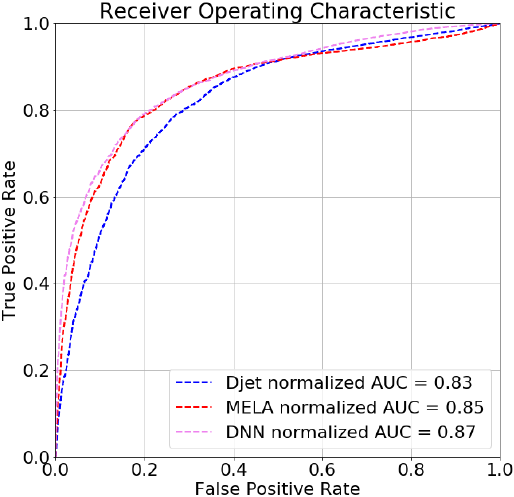
\includegraphics[width=0.3\textwidth]{figs/3jets_pt_eta_phi_no_weight_vbf_vs_all_leptons_sorting_issue}
	\quad
	\quad
	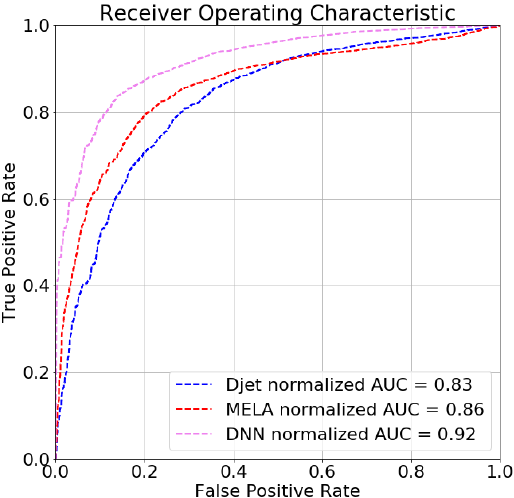
\includegraphics[width=0.3\textwidth]{figs/3jets_pt_eta_phi_weight_sum_vbf_vs_all_leptons_sorting_issue}
	\caption{ROC curves comparing the performance of a trained NN, the VBF MELA discriminant and $D_{jet}$: (a) the performance of NN without scaling the \textit{loss} and (b) performance after scaling the \textit{loss}.}
	\label{fig:scaling_training_effect}
\end{figure}

\end{document}          
